\chapter{Results}\label{ch:results}
In this chapter the results of the simulation will be shown.


The goal of this simulation is to simulate a daily flow in the northern part of Fredericia, where the disturbance can be seen on the input to the WWTP. To do so the simulation model explained in \ref{ch:simulation} is utilized. However, the pump station, illustrated with the blue solid circle in figure \ref{fig:kloakgrid}, is not included in this simulation, as it will smooth the flow from that station down to the WWTP, thus there will not be any variation in the flow into the WWTP. To generate the disturbances from the residential and industrial zones, shown in figure \ref{fig:kloakgrid_simplified}, the flow profiles in appendix \ref{app:flow_profiles} is used. These disturbance models are not simulated from the zones into the main sewer line, but are directly added on the main sewer line, therefore causing higher peaks. It has been chosen to only use the disturbance from the brewery and bottling plant, as the data from the refinery is not accessible. The disturbance from the brewery and bottling plant is shown in figure \ref{fig:flow_profile_industry}. The pipe specifications for this simulation can be seen in table \ref{tab:pipe_data_nonlinear_linear_testv2}.  
\begin{table}[H]
\centering
\begin{tabular}{|c|c|c|c|c|c|c|c|}
\hline
\begin{tabular}[c]{@{}c@{}}Component\\ number\end{tabular} & Length {[}m{]} & Sections & Dx {[}m{]} & Ib     & d {[}m{]} & $\theta$ & \begin{tabular}[c]{@{}c@{}}$Q_f $\\  {[}$m^3/s${]}\end{tabular} \\ \hline
1                                                          & 700            & 35       & 20         & 0,003  & 0,9       & 0,65     & 0,972                                                                          \\ \hline
3                                                          & 303            & 15       & 20,2       & 0,003  & 0,9       & 0,65     & 0,972                                                                          \\ \hline
4                                                          & 27             & 1        & 27         & 0,003  & 1         & 0,65     & 1,284                                                                          \\ \hline
5                                                          & 155            & 8        & 19,4       & 0,0041 & 1         & 0,65     & 1,50                                                                           \\ \hline
6                                                          & 295            & 14       & 21         & 0,0122 & 0,8       & 0,65     & 1,438                                                                          \\ \hline
7                                                          & 318            & 15       & 21,2       & 0,0053 & 0,9       & 0,65     & 1,293                                                                          \\ \hline
8                                                          & 110            & 5        & 22         & 0,0036 & 0,9       & 0,65     & 1,066                                                                          \\ \hline
9                                                          & 38             & 2        & 19         & 0,0024 & 1         & 0,65     & 1,149                                                                          \\ \hline
10                                                         & 665            & 30       & 22,2       & 0,003  & 1         & 0,65     & 1,284                                                                          \\ \hline
11                                                         & 155            & 7        & 22,1       & 0,0008 & 1         & 0,65     & 0,663                                                                          \\ \hline
12                                                         & 955            & 40       & 23,9       & 0,0029 & 1,2       & 0,65     & 2,041                                                                          \\ \hline
13                                                         & 304            & 15       & 20,3       & 0,003  & 1,2       & 0,65     & 2,076                                                                          \\ \hline
14                                                         & 116            & 5        & 23,2       & 0,0021 & 1,2       & 0,65     & 1,737                                                                          \\ \hline
15                                                         & 283            & 12       & 23,6       & 0,0017 & 1,4       & 0,65     & 2,346                                                                          \\ \hline
16                                                         & 31             & 1        & 31         & 0,0019 & 1,4       & 0,65     & 2,480                                                                          \\ \hline
17                                                         & 125            & 6        & 20,8       & 0,0021 & 1,6       & 0,65     & 3,707                                                                          \\ \hline
18                                                         & 94             & 4        & 23,5       & 0,0013 & 1,5       & 0,65     & 2,461                                                                          \\ \hline
19                                                         & 360            & 15       & 24         & 0,0046 & 1,6       & 0,65     & 5,487                                                                          \\ \hline
20                                                         & 736            & 32       & 23         & 0,0012 & 1,6       & 0,65     & 2,802                                                                          \\ \hline
\end{tabular}
\caption{The specification of the pipes for in the simulation.}
\label{tab:pipe_data_nonlinear_linear_testv2}
\end{table}

The tank specification can be seen in table \ref{tab:tank_data_nonlinear_linear_testv2}.

\begin{table}[H]
\centering
\begin{tabular}{|c|c|}
\hline
\begin{tabular}[c]{@{}c@{}}Component\\ number\end{tabular} & 2  \\ \hline
Size $[m^3]$                                              & 90 \\ \hline
Height {[}m{]}                                             & 10 \\ \hline
Area {[}$m^2$                                              & 9  \\ \hline
\end{tabular}
\caption{The tank specification for the simulation. }
\label{tab:tank_data_nonlinear_linear_testv2}
\end{table}

Furthermore, table \ref{tab:system_setup_nonlinear_linear_test} shows the system setup.

\begin{table}[H]
\centering
\begin{tabular}{|c|c|c|}
\hline
Type  & Component & Sections \\ \hline
Pipe  & 1         & 35       \\ \hline
Tank  & 1         & 1        \\ \hline
Pipe  & 18        & 227      \\ \hline
Total & 20        & 263      \\ \hline
\end{tabular}
\caption{The system setup.}
\label{tab:system_setup_nonlinear_linear_testv2}
\end{table}

Where the first component in the simulated sewer network is a pipe followed by a tank and hereafter 18 pipes follows. The first pipe and the tank have been added on the originally sewer network shown in figure \ref{fig:sewer_line_diagram}. The first pipe goes from the larger industrial area down to the main sewer line showed with a black circle in figure \ref{fig:kloakgrid_simplified}, where the tank is placed as well. The reason for placing the tank there is, that the idea would have been to smoothen the wastewater coming from the larger industry. Furthermore, the pipe is placed, as the MPC could have used it for prediction, as it would be able to measure the disturbance going into the pipe at the industry, and thereby use it in the predictive model to calculate the must optimal control output to the pump. However, as this it not possible, due to the MPC controller is not able to keep a flow output, where the flow variations are kept to a minimum, and as the prediction horizon is limited due to non-convexity as explained in section \ref{se:model_predictive_control}. Therefore in the simulation the tank will just transfer wastewater from the previous pipe to the pipe after the tank. 

Several simulation was conducted to find the must optimal $\Delta t$ as explained in section \ref{subse:stability_and_precision}. As the pipes are split in different sections and as the average flow height is also different from pipe to pipe. Therefore the Courant number variates from pipe to pipe, and is therefore difficult to tune so all pipes have the must optimal Courant number. However, it was found that a $\Delta t = 20$, with the given $\Delta x$ shown in table \ref{tab:pipe_data_nonlinear_linear_testv2}, gave the must realistic outcome, as values lower resulted in a output where some distortion was visible.

In figure \ref{fig:simulation_output_first} the output of a simulation across two days are shown. 

\begin{figure}[H]
\centering
% This file was created by matlab2tikz.
%
%The latest updates can be retrieved from
%  http://www.mathworks.com/matlabcentral/fileexchange/22022-matlab2tikz-matlab2tikz
%where you can also make suggestions and rate matlab2tikz.
%
\definecolor{mycolor1}{rgb}{0.00000,0.44700,0.74100}%
%
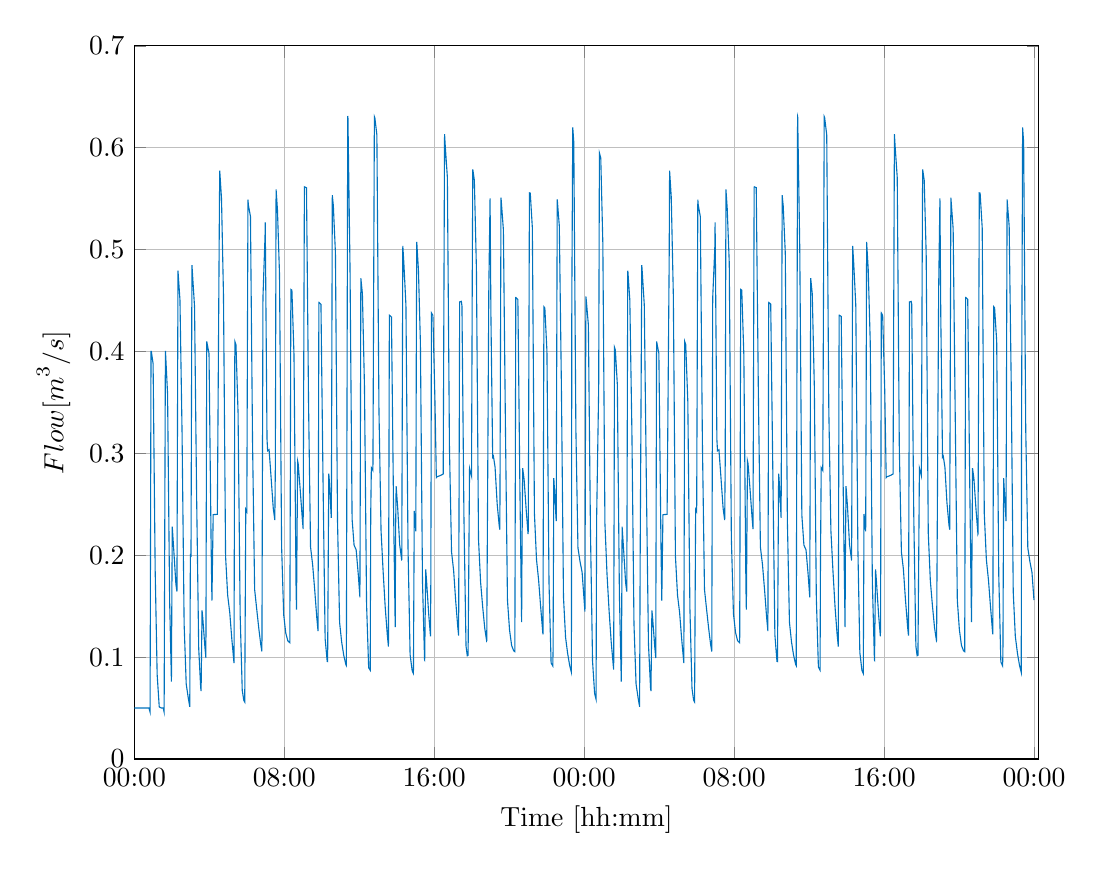
\begin{tikzpicture}

\begin{axis}[%
width=4.521in,
height=3.566in,
at={(0.758in,0.481in)},
scale only axis,
xmin=1,
scaled x ticks = false,
xmajorgrids,
ymajorgrids,
xmax=173664,
xtick={1,28801,57601,86401,115201,144001,172801},
xticklabels={{00:00},{08:00},{16:00},{00:00},{08:00},{16:00},{00:00},{},{},{}},
xlabel={Time [hh:mm]},
ymin=0,
ymax=0.7,
ylabel={$\text{Flow [m}^\text{3}\text{/s]}$},
axis background/.style={fill=white}
]
\addplot [color=mycolor1,solid,forget plot]
  table[row sep=crcr]{%
1	0.0499997152763342\\
381	0.0499999892074085\\
681	0.0499999887402718\\
781	0.0499999900942177\\
801	0.0499999900283255\\
1081	0.049999984018313\\
1261	0.0499999893262727\\
1521	0.0499999838340426\\
1601	0.049999984809447\\
2001	0.0499999906588171\\
2061	0.0499999922125646\\
2401	0.049999988996632\\
2781	0.0499999918475296\\
2801	0.0499999801986038\\
3021	0.0460373492555953\\
3201	0.39999620912548\\
3261	0.399999964024236\\
3601	0.388038894071086\\
4001	0.184947858626601\\
4381	0.082805088531536\\
4781	0.0511451879298567\\
5181	0.0500002487860619\\
5541	0.0499999248577416\\
5721	0.0460373452553259\\
5961	0.399999974821009\\
5981	0.399999971271513\\
6381	0.358516455127467\\
6781	0.154383868746348\\
7121	0.0760256189325568\\
7181	0.13826974014641\\
7281	0.228026620985396\\
7581	0.204239805785136\\
7981	0.171590440555943\\
8181	0.164315181527722\\
8381	0.47926934050765\\
8761	0.450413278243777\\
9161	0.321534576651487\\
9561	0.132277730995904\\
9961	0.0735649221955217\\
10361	0.0597071439387407\\
10641	0.0512695775424259\\
10761	0.20005447478489\\
10881	0.199434615905679\\
11061	0.48473586623314\\
11161	0.476723871738909\\
11561	0.443897750738214\\
11961	0.25806849480281\\
12361	0.108844325174995\\
12741	0.0700275093087758\\
12821	0.0667206908995504\\
13001	0.145928679109392\\
13141	0.138393729441425\\
13541	0.110667079625233\\
13741	0.0991507389943454\\
13901	0.40986305875768\\
13941	0.40882623802115\\
14341	0.398007217901318\\
14741	0.212131825065823\\
14901	0.155368306478837\\
15141	0.239872608579426\\
15541	0.240004691937102\\
15941	0.240038886655287\\
16341	0.543707035296884\\
16401	0.577386156049016\\
16741	0.5499489464615\\
17121	0.454515865313659\\
17521	0.199211784759613\\
17921	0.160813386913845\\
18321	0.143916888943139\\
18721	0.117703671201611\\
19121	0.095049498732015\\
19141	0.0940665657039142\\
19301	0.409784435964215\\
19521	0.406501876116627\\
19921	0.33935537668123\\
20321	0.141804797058712\\
20721	0.067435176520201\\
21021	0.0575846925747079\\
21201	0.0559457131457851\\
21401	0.244991184003057\\
21601	0.242763538199487\\
21821	0.5490148580277\\
21901	0.543815970276843\\
22301	0.532449053725931\\
22701	0.311242442063504\\
23101	0.166455067970211\\
23501	0.147143722635203\\
23901	0.128218569971245\\
24301	0.111515660096113\\
24501	0.105546274424128\\
24701	0.452877166239096\\
25101	0.513490813859022\\
25141	0.526641040406919\\
25481	0.314069608587414\\
25601	0.302486128983783\\
25881	0.303568709699798\\
26281	0.275044058907798\\
26681	0.245964195626756\\
26981	0.234447696691942\\
27081	0.288110624118585\\
27221	0.559006245862765\\
27481	0.539613674285018\\
27881	0.475567692570443\\
28281	0.209018911404775\\
28681	0.141668747218986\\
29081	0.123608641874535\\
29481	0.11592694443507\\
29861	0.114080220104003\\
30061	0.460896204122244\\
30261	0.460167448207798\\
30661	0.396678419054452\\
31061	0.168157104268696\\
31141	0.146550603859365\\
31361	0.292440612392119\\
31461	0.290155884720642\\
31861	0.26381450895376\\
32261	0.23554830781087\\
32421	0.225714221407563\\
32661	0.561584147546688\\
33061	0.560624758930501\\
33461	0.348105695677251\\
33841	0.208065283311125\\
34241	0.190782917669544\\
34641	0.166025134280847\\
35041	0.13873822553377\\
35281	0.125451644802619\\
35441	0.4478352243038\\
35461	0.44811407769246\\
35841	0.446214141629251\\
36241	0.27225617680166\\
36641	0.118110855826106\\
37041	0.095767561962741\\
37121	0.0956553614348974\\
37341	0.280096449864026\\
37441	0.273855912758517\\
37821	0.236596990821348\\
37841	0.237774941596493\\
38021	0.553366894967955\\
38221	0.54291518952707\\
38621	0.49660305179753\\
39021	0.233847581211315\\
39421	0.134033881707084\\
39821	0.114649017608518\\
40221	0.101701052031103\\
40621	0.0927146992547936\\
40721	0.0917383187540116\\
40981	0.63107071951054\\
41021	0.630035704702444\\
41421	0.482341851596278\\
41821	0.235563366290832\\
42201	0.209832049584584\\
42601	0.205284923234108\\
43001	0.181573721441432\\
43321	0.158651139798747\\
43401	0.287395033266756\\
43501	0.471956377710797\\
43801	0.456578916341174\\
44201	0.364798527107059\\
44601	0.151919551074707\\
45001	0.0895967214260026\\
45301	0.0871144475971674\\
45401	0.241707281322062\\
45521	0.285948268035892\\
45821	0.283146889932263\\
46101	0.630469173265171\\
46201	0.629088537957435\\
46581	0.612545920500935\\
46981	0.342528955023114\\
47381	0.224203484709649\\
47781	0.184153073081266\\
48181	0.149030782566006\\
48581	0.12195593910867\\
48801	0.110280587955104\\
48981	0.435567061037672\\
49381	0.433837256348174\\
49781	0.247137117278272\\
50101	0.129323544894529\\
50181	0.226587016813804\\
50281	0.267899772040847\\
50581	0.246318904302867\\
50961	0.210314398331763\\
51341	0.195657253277077\\
51361	0.195784009404707\\
51561	0.503592036774015\\
51761	0.486974841272141\\
52161	0.445428690023276\\
52561	0.207716541625214\\
52961	0.102502304765683\\
53361	0.0865204262570826\\
53601	0.0839471479111217\\
53761	0.243524692542883\\
54061	0.22335472358936\\
54161	0.413641605154435\\
54241	0.507566556159231\\
54561	0.48007415997152\\
54941	0.408444008474248\\
55341	0.174114153859742\\
55741	0.0971405673619263\\
55761	0.096975498915427\\
55961	0.186119510987269\\
56141	0.173353292951344\\
56541	0.141804669337536\\
56881	0.120312676919824\\
56941	0.17363089926247\\
57061	0.437782042398014\\
57341	0.435474087380637\\
57741	0.350377749978731\\
58001	0.276216298585415\\
58141	0.277039370834222\\
58541	0.277740752111343\\
58941	0.278635286488113\\
59321	0.279736664395953\\
59581	0.613239888945005\\
59721	0.601155920090224\\
60121	0.570829618399022\\
60521	0.30525522703366\\
60921	0.203256919582693\\
61321	0.185129585157137\\
61721	0.154979527639579\\
62121	0.129229876043253\\
62281	0.12114747426953\\
62481	0.44862995078268\\
62801	0.449171273418054\\
62921	0.444677955276041\\
63301	0.237964284751834\\
63701	0.111008795041031\\
63941	0.101319095647373\\
64101	0.101831871303562\\
64381	0.285451159479523\\
64761	0.277800728120848\\
64901	0.472346688429331\\
65001	0.578732309508892\\
65301	0.568128800263333\\
65701	0.480556114992309\\
66101	0.215435701651473\\
66501	0.173587977353262\\
66901	0.149411121057409\\
67301	0.128194088457934\\
67661	0.115879979337036\\
67681	0.116080976474654\\
68081	0.463231310412606\\
68321	0.550240918542084\\
68481	0.43704169328213\\
68821	0.296195131686067\\
68961	0.297296204143991\\
69281	0.286349521684829\\
69681	0.250540179409776\\
70081	0.228693231365457\\
70201	0.225059553792036\\
70421	0.550888655859785\\
70481	0.546993291279657\\
70881	0.519239767321056\\
71281	0.321893080651539\\
71661	0.155884099827311\\
72061	0.126611870338134\\
72461	0.111441871585865\\
72861	0.106140611089357\\
73081	0.105332967336101\\
73261	0.452946083990718\\
73281	0.453024300871342\\
73661	0.451074937198832\\
74061	0.26082900810748\\
74381	0.134237338321971\\
74461	0.207813944879953\\
74581	0.285378186391529\\
74861	0.274285223507388\\
75261	0.244391347849864\\
75621	0.220651866001535\\
75661	0.224809763811749\\
75881	0.5556579938168\\
76041	0.555440125466322\\
76441	0.52143634234302\\
76841	0.240745754972094\\
77241	0.195680996475161\\
77641	0.175811605109868\\
78041	0.149008733822511\\
78441	0.124162090755598\\
78481	0.122293389503727\\
78661	0.44384907080836\\
78841	0.442708151044371\\
79241	0.400372910545192\\
79641	0.172855897377427\\
80041	0.0943411879687305\\
80361	0.0913677029693039\\
80421	0.105748914607317\\
80561	0.275622277873239\\
81021	0.233525034544167\\
81221	0.549299988830962\\
81621	0.523015869588244\\
82021	0.365589134600443\\
82421	0.158832345842062\\
82821	0.119381319389791\\
83221	0.103510284822917\\
83621	0.0914259162743653\\
83941	0.0850821629137212\\
84021	0.449966203224246\\
84201	0.619938777189986\\
84401	0.605215327407337\\
84801	0.323950052106171\\
85201	0.207162769487388\\
85601	0.193722933184863\\
86001	0.183208432749678\\
86401	0.154546451194393\\
86541	0.144709226768709\\
86721	0.454054707630259\\
86801	0.450268450488853\\
87201	0.426082168190829\\
87601	0.224018825746384\\
88001	0.0961050037604321\\
88401	0.0642514476254031\\
88681	0.058588377418986\\
88781	0.233884823055304\\
89181	0.363764232190534\\
89321	0.594800267880994\\
89581	0.589951272879468\\
89981	0.505665048374919\\
90381	0.231007553197322\\
90781	0.181446768847678\\
91181	0.145374472013491\\
91581	0.115191653805948\\
91981	0.0918291899207325\\
92061	0.0877953189909785\\
92221	0.403907758239193\\
92381	0.401514711023063\\
92761	0.367814281450466\\
93161	0.161459811427181\\
93521	0.0760258697047347\\
93561	0.0969253175283628\\
93681	0.228026635800281\\
93961	0.206157068010913\\
94361	0.172716138741509\\
94581	0.164315181527722\\
94761	0.477771577804068\\
94781	0.47926934050765\\
95161	0.450413278243778\\
95561	0.321534576651487\\
95961	0.132277730995905\\
96361	0.0735649221955217\\
96761	0.0597071439387407\\
97041	0.0512695775424261\\
97141	0.189954342640788\\
97461	0.48473586623314\\
97541	0.478621526310808\\
97941	0.445565551010111\\
98341	0.270052824073967\\
98741	0.112972942133323\\
99141	0.0700275093087758\\
99221	0.0667206908995504\\
99401	0.145928679109392\\
99541	0.138393729441425\\
99941	0.110667079625233\\
100141	0.0991507389943454\\
100301	0.40986305875768\\
100341	0.40882623802115\\
100741	0.398007217901318\\
101141	0.212131825065823\\
101301	0.155368306478837\\
101521	0.239674727124832\\
101921	0.240004160488744\\
102321	0.240032761489357\\
102721	0.490613201150536\\
102801	0.577385614042946\\
103121	0.551397788492204\\
103521	0.454515521091378\\
103921	0.199211766547411\\
104321	0.160811738559319\\
104721	0.143916519077449\\
105121	0.117702397972358\\
105501	0.0960563302766093\\
105541	0.0940655608631718\\
105701	0.409782142347942\\
105901	0.406701240316587\\
106301	0.350756062230757\\
106701	0.148179236245713\\
107101	0.0692618286459731\\
107421	0.0575801460066641\\
107601	0.0559429268585551\\
107801	0.244982676605651\\
108001	0.242757068811194\\
108221	0.54900476716055\\
108301	0.543808297503321\\
108701	0.532436480925017\\
109101	0.311241030199004\\
109501	0.166447159541348\\
109881	0.14801645052783\\
110281	0.129144882903335\\
110681	0.112225593742404\\
110901	0.105541387787785\\
111081	0.452627367523953\\
111481	0.501364815585408\\
111541	0.526586805232183\\
111881	0.314064927206939\\
112001	0.302477482482032\\
112281	0.303564415396613\\
112681	0.275045931553673\\
113081	0.245964222909356\\
113381	0.234448498754518\\
113481	0.288116696094247\\
113621	0.559006398210286\\
113861	0.540979121709231\\
114261	0.486855270635058\\
114661	0.217493518570819\\
115061	0.142802563645621\\
115461	0.124291854749527\\
115861	0.116093137321325\\
116261	0.114084290390741\\
116461	0.460899377915235\\
116661	0.460171947548487\\
117061	0.396679285152434\\
117461	0.168158461755987\\
117541	0.146555138425319\\
117761	0.292445572598367\\
117861	0.290159181668251\\
118241	0.265401886805784\\
118641	0.236956301886082\\
118821	0.225714522330167\\
119041	0.561469488609575\\
119061	0.561586041554716\\
119441	0.560805439144691\\
119841	0.363932228586388\\
120241	0.208067125535311\\
120641	0.190785255682231\\
121041	0.166025588105298\\
121441	0.13873932167539\\
121681	0.125453388188775\\
121841	0.447837563995478\\
121861	0.448116051383338\\
122221	0.4464561479952\\
122621	0.284824476239217\\
123021	0.121970167931679\\
123421	0.0958081500032729\\
123521	0.0956573749864267\\
123741	0.280096851577685\\
123821	0.275531608454023\\
124221	0.236598409026601\\
124421	0.553367619300467\\
124621	0.5429157709688\\
125021	0.496603413412628\\
125421	0.233847680410384\\
125821	0.134033685469667\\
126221	0.114650333534502\\
126601	0.102289103709303\\
127001	0.0929882528747439\\
127121	0.0917392868371645\\
127381	0.631071912873843\\
127401	0.630719116657667\\
127801	0.501347161814062\\
128201	0.239397450469059\\
128601	0.209832888971714\\
129001	0.205285541414406\\
129401	0.181574246023112\\
129721	0.158651581187078\\
129801	0.287397627582394\\
129901	0.471956617871342\\
130201	0.456579492165227\\
130601	0.364798643465493\\
130981	0.158461721428025\\
131381	0.0902446213392131\\
131701	0.0871147730920042\\
131781	0.195332180975037\\
131921	0.285946978271874\\
132221	0.283146011645084\\
132501	0.630469563534361\\
132581	0.62947257325151\\
132981	0.612546279103266\\
133381	0.342529069488647\\
133781	0.22420331583186\\
134181	0.18415338411579\\
134581	0.149030236035514\\
134961	0.123132349572876\\
135201	0.110280603793395\\
135361	0.435176913377614\\
135381	0.435567198316332\\
135761	0.434402963450522\\
136161	0.258663077151003\\
136501	0.129324848709165\\
136561	0.193972315730123\\
136681	0.267900152487372\\
136961	0.248282666486158\\
137361	0.210314788420516\\
137741	0.195657673398787\\
137761	0.195784442440667\\
137961	0.503592296507298\\
138161	0.48697576182077\\
138561	0.445428205217198\\
138961	0.207716601935443\\
139341	0.104535524709347\\
139741	0.0868948301247878\\
140001	0.0839475146696737\\
140141	0.240432040289202\\
140461	0.223354613707161\\
140541	0.341067258228241\\
140641	0.507566355305644\\
140941	0.481669135095204\\
141341	0.408443854052323\\
141741	0.174114080843233\\
142141	0.0971401552400959\\
142161	0.0969748967063283\\
142361	0.186118838354968\\
142541	0.173352807110823\\
142941	0.141804218930691\\
143281	0.120311786985649\\
143321	0.129127350722078\\
143461	0.437780930522792\\
143721	0.435517651687087\\
144121	0.361960854279469\\
144401	0.276209489946611\\
144521	0.277012003580165\\
144921	0.277695129632075\\
145321	0.278586129391934\\
145721	0.279729241245801\\
145981	0.613237806000591\\
146121	0.601153312486374\\
146521	0.570827166257067\\
146921	0.305254463448292\\
147321	0.20325470575301\\
147701	0.186543247083285\\
148101	0.15643029351033\\
148501	0.130357894127212\\
148681	0.121144762304623\\
148881	0.448629034177187\\
149201	0.449165808875287\\
149301	0.446696179355606\\
149701	0.237965618956237\\
150101	0.111008331346555\\
150341	0.101316327092596\\
150501	0.101826939135492\\
150781	0.285447611650934\\
151161	0.27779589570848\\
151301	0.472339570784934\\
151401	0.578729951396445\\
151701	0.568123276721063\\
152081	0.495832401738009\\
152481	0.221821174469093\\
152881	0.17473208468221\\
153281	0.150604920464296\\
153681	0.12910065597234\\
154061	0.115878791323534\\
154081	0.116079655938807\\
154481	0.463229573529833\\
154721	0.5502375854001\\
154881	0.437041948039623\\
155221	0.296195355930144\\
155361	0.297296933741909\\
155681	0.286350503920018\\
156061	0.252102910380496\\
156461	0.229497997298456\\
156601	0.225064130916765\\
156821	0.550890260513285\\
156861	0.548562055547551\\
157261	0.520520415207785\\
157661	0.336720865555416\\
158061	0.155883549287124\\
158461	0.126615126562859\\
158861	0.111443479804903\\
159261	0.106144927681463\\
159481	0.105335017541325\\
159661	0.452949294313543\\
159681	0.453027104859375\\
160061	0.451077022810141\\
160441	0.272986614049946\\
160781	0.134240624188618\\
160841	0.171194243932062\\
160981	0.285380797796743\\
161241	0.27560958645801\\
161641	0.245748272441495\\
162021	0.22065246306675\\
162041	0.22095872866312\\
162281	0.555659486202346\\
162441	0.555441569380212\\
162841	0.521436911503331\\
163241	0.240744945577966\\
163641	0.195682416129531\\
164041	0.175812474037148\\
164421	0.150374209915759\\
164821	0.125268272587349\\
164881	0.122293793898792\\
165061	0.443850629799895\\
165221	0.442791980296207\\
165621	0.41026583231508\\
166021	0.18061579852657\\
166421	0.0952920563520666\\
166761	0.09137016735018\\
166821	0.105761024965842\\
166961	0.275625277048089\\
167421	0.233525909462804\\
167621	0.549302071760907\\
168021	0.523017665432503\\
168421	0.365587501813481\\
168801	0.163841775577553\\
169201	0.120372383531068\\
169601	0.10417680851964\\
170001	0.0919608721649096\\
170341	0.0850844928164687\\
170401	0.33174516873495\\
170601	0.619937197264595\\
170801	0.605220107773325\\
171201	0.323949146474474\\
171601	0.207163720135008\\
172001	0.193730162139822\\
172401	0.183213876546389\\
172781	0.156061090616425\\
};
\end{axis}
\end{tikzpicture}%
\caption{Output of the last pipe into the WWTP.}
\label{fig:simulation_output_first}
\end{figure}  

It is clear that flow variates to a great extent as is also shown in figure \ref{fig:flow_input_wwtp} from the WWTP at Fredericia. However, these two can not be direct compared, as the data from Fredericia also includes the wastewater from the southern part of the city. But can give a indication that the simulation correspond to what is happening in the reality. However, the simulated results in a greater variation of flow than the data obtained from Fredericia. This could be due to the pump, as mention previously, that it smoothen the flow from the northern part of the city and therefore the variations on the figure from Fredericia is due to disturbance coming from the southern part of the city.       

